
\section*{ANNEXES}
\addcontentsline{toc}{section}{ANNEXES}

\subsection*{Annexe A — Captures d'écran}
\addcontentsline{toc}{subsection}{Annexe A — Captures d'écran}

% Remplacer chaque cadre par \includegraphics après ajout du fichier indiqué.

\begin{figure}[h!]
    \centering
    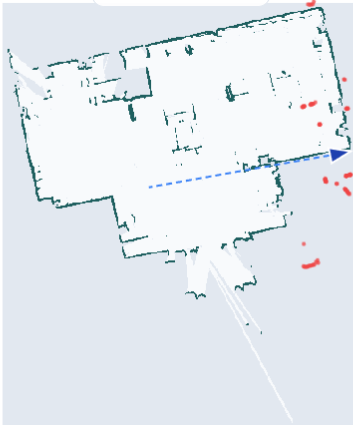
\includegraphics[width=0.8\textwidth]{captures_ecran/Capture1.png}
    \caption{Carte SLAM du laboratoire — interface opérateur
    (\texttt{captures\_ecran/Capture1.png})}
    \label{fig:annexe_carte}
\end{figure}

\begin{figure}[h!]
    \centering
    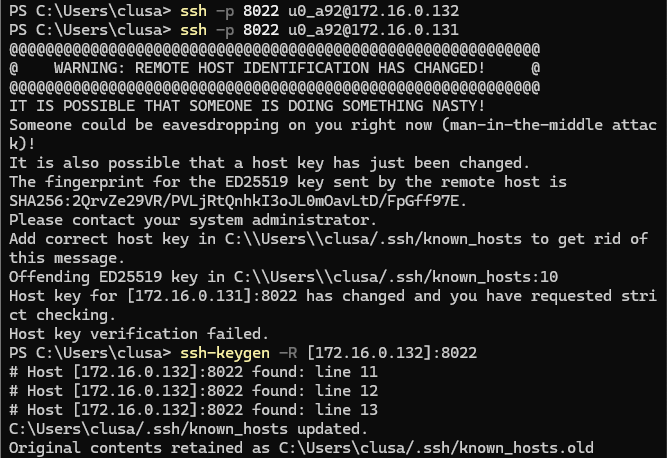
\includegraphics[width=0.8\textwidth]{captures_ecran/Capture2.png}
    \caption{Terminal — vérification de connectivité
    (\texttt{captures\_ecran/Capture2.png})}
    \label{fig:annexe_terminal}
\end{figure}

\begin{figure}[h!]
    \centering
    \fbox{\parbox{0.75\textwidth}{\centering\vspace{2.5cm}
    \textit{Capture à insérer}\\[0.3cm]
    \texttt{captures\_ecran/dashboard\_operateur.png}\vspace{2.5cm}}}
    \caption{Dashboard opérateur — mode robot réel \textit{(à insérer)}}
    \label{fig:annexe_dashboard}
\end{figure}

\begin{figure}[h!]
    \centering
    \fbox{\parbox{0.75\textwidth}{\centering\vspace{2.5cm}
    \textit{Capture à insérer}\\[0.3cm]
    \texttt{captures\_ecran/panneau\_visite.png}\vspace{2.5cm}}}
    \caption{Panneau visite guidée — page Visite \textit{(à insérer)}}
    \label{fig:annexe_visite}
\end{figure}

\begin{figure}[h!]
    \centering
    \fbox{\parbox{0.75\textwidth}{\centering\vspace{2.5cm}
    \textit{Capture à insérer}\\[0.3cm]
    \texttt{captures\_ecran/kiosque\_accueil.png}\vspace{2.5cm}}}
    \caption{Kiosque visiteur — écran d'accueil FR \textit{(à insérer)}}
    \label{fig:annexe_kiosque_accueil}
\end{figure}

\begin{figure}[h!]
    \centering
    \fbox{\parbox{0.75\textwidth}{\centering\vspace{2.5cm}
    \textit{Capture à insérer}\\[0.3cm]
    \texttt{captures\_ecran/kiosque\_running.png}\vspace{2.5cm}}}
    \caption{Kiosque visiteur — visite en cours \textit{(à insérer)}}
    \label{fig:annexe_kiosque_running}
\end{figure}

\begin{figure}[h!]
    \centering
    \fbox{\parbox{0.75\textwidth}{\centering\vspace{2.5cm}
    \textit{Capture à insérer}\\[0.3cm]
    \texttt{captures\_ecran/erreur\_604.png}\vspace{2.5cm}}}
    \caption{Erreur de navigation 604 sur tablette \textit{(à insérer)}}
    \label{fig:annexe_erreur_604}
\end{figure}

\begin{figure}[h!]
    \centering
    \fbox{\parbox{0.75\textwidth}{\centering\vspace{2.5cm}
    \textit{Capture à insérer}\\[0.3cm]
    \texttt{captures\_ecran/apk\_tablette.png}\vspace{2.5cm}}}
    \caption{Application \texttt{CybelVisitorKiosk} sur tablette \textit{(à insérer)}}
    \label{fig:annexe_apk}
\end{figure}

\subsection*{Annexe B — Dépôt source du projet}
\addcontentsline{toc}{subsection}{Annexe B — Dépôt source du projet}

\begin{itemize}
    \item \textbf{Dépôt principal CYBEL} (branche \texttt{main}) :\\
    \url{https://github.com/Claude20022002/Projet-Stage-2026-Cybel}
    \item \textbf{Branche chatbot} (G. Khalifi) :\\
    \url{https://github.com/Claude20022002/Projet-Stage-2026-Cybel/tree/chatbot-cybel-projet-2026}
\end{itemize}

\subsection*{Annexe C — Commandes utiles}
\addcontentsline{toc}{subsection}{Annexe C — Commandes utiles}

\begin{lstlisting}[style=terminal, language=bash, caption={Commandes PC (PowerShell)}]
# Verification reseau
ping 10.42.0.1
python scripts\robot_status.py

# Lancement developpement
python scripts\dev.py

# Tests unitaires (78 tests)
python -m pytest tests/ -v

# TTS test (USB branche)
adb shell am broadcast -n com.cybel.ttsbridge/.SpeakReceiver ^
  -a com.cybel.ttsbridge.SPEAK --es text "Test HESTIM"

# Deploiement tablette
python scripts\deploy_termux.py --skip-kiosk-build --lite-only --host <IP>
\end{lstlisting}

\begin{lstlisting}[style=terminal, language=bash, caption={Commandes Termux (tablette)}]
cd ~/cybel/scripts/termux
./stop_cybel.sh && ./start_cybel.sh
curl http://127.0.0.1:8000/api/health
\end{lstlisting}

\subsection*{Annexe D — Extraits de code significatifs}
\addcontentsline{toc}{subsection}{Annexe D — Extraits de code significatifs}

\paragraph{D.1 — Annulation de navigation (\texttt{sdk/real\_robot.py}).}

\begin{verbatim}
async def _cancel_navigation(self) -> None:
    for args in [{"command": "stop"}, ...]:
        await self._client.call_service(
            ROS_SERVICES["poi"], args, timeout=3.0)
    await call_service_first(self._client, ...)
    await self._publish_velocity(0.0, 0.0)
\end{verbatim}

\paragraph{D.2 — Publication d'un objectif de navigation.}

\begin{verbatim}
await self._client.publish(ROS_TOPICS["navi_goal"], {
    "header": {"frame_id": "map"},
    "pose": {
        "position": {"x": x, "y": y, "z": 0.0},
        "orientation": {"z": sin(theta/2), "w": cos(theta/2)},
    },
})
\end{verbatim}

\paragraph{D.3 — Structure d'un arrêt (\texttt{data/lab\_tour.json}).}

\begin{verbatim}
{
  "id": "cnc_router",
  "equipment_fr": "Routeur CNC",
  "x": -8.38, "y": 1.45, "theta": 0.88,
  "speech_fr": "Le routeur CNC permet d'usiner...",
  "dwell_seconds": 12
}
\end{verbatim}

\subsection*{Annexe E — Diagrammes détaillés}
\addcontentsline{toc}{subsection}{Annexe E — Diagrammes détaillés}

Sources Mermaid dans \texttt{docs/Sujet de stage/diagrammes/} du dépôt CYBEL.
Remplacer chaque cadre par \texttt{\textbackslash includegraphics} après export PNG.

\begin{figure}[h!]
    \centering
    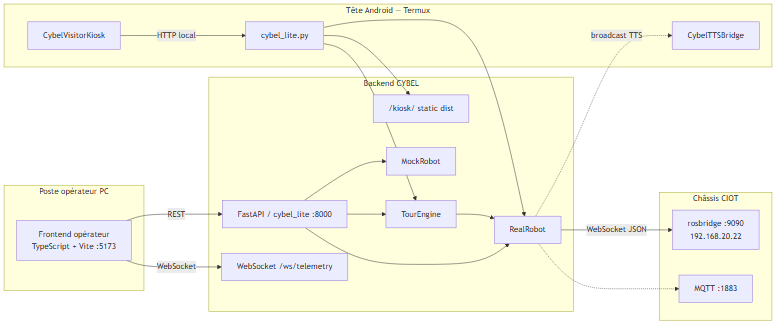
\includegraphics[width=0.85\textwidth]{diagramme/diagramme_composant.png}
    \caption{Diagramme de composants
    (\texttt{diagramme/diagramme\_composant.png})}
    \label{fig:annexe_composants}
\end{figure}

\begin{figure}[h!]
    \centering
    \fbox{\parbox{0.75\textwidth}{\centering\vspace{2.5cm}
    \textit{Diagramme à insérer}\\[0.3cm]
    \texttt{diagramme/architecture\_couches.png}\vspace{2.5cm}}}
    \caption{Architecture en couches \textit{(à insérer)}}
    \label{fig:annexe_archi_couches}
\end{figure}

\begin{figure}[h!]
    \centering
    \fbox{\parbox{0.75\textwidth}{\centering\vspace{2.5cm}
    \textit{Diagramme à insérer}\\[0.3cm]
    \texttt{diagramme/topologie\_reseau.png}\vspace{2.5cm}}}
    \caption{Topologie réseau du robot \textit{(à insérer)}}
    \label{fig:annexe_topologie}
\end{figure}

\begin{figure}[h!]
    \centering
    \fbox{\parbox{0.75\textwidth}{\centering\vspace{2.5cm}
    \textit{Diagramme à insérer}\\[0.3cm]
    \texttt{diagramme/sequence\_lab\_tour.png}\vspace{2.5cm}}}
    \caption{Séquence — visite guidée laboratoire \textit{(à insérer)}}
    \label{fig:annexe_seq_tour}
\end{figure}

\begin{figure}[h!]
    \centering
    \fbox{\parbox{0.75\textwidth}{\centering\vspace{2.5cm}
    \textit{Diagramme à insérer}\\[0.3cm]
    \texttt{diagramme/sequence\_tts.png}\vspace{2.5cm}}}
    \caption{Séquence — synthèse vocale (TTS) \textit{(à insérer)}}
    \label{fig:annexe_seq_tts}
\end{figure}

\subsection*{Annexe F — Documentation technique complémentaire}
\addcontentsline{toc}{subsection}{Annexe F — Documentation technique complémentaire}

\begin{table}[h!]
\centering
\caption{Index de la documentation technique CYBEL}
\begin{tabular}{|p{5cm}|p{8cm}|}
\hline
\textbf{Document} & \textbf{Chemin dans le dépôt} \\
\hline
README projet & \texttt{README.md} \\
\hline
Guide interface opérateur & \texttt{docs/INTERFACE.md} \\
\hline
Pont TTS & \texttt{docs/TTS\_BRIDGE.md} \\
\hline
Kiosque visiteur & \texttt{docs/VISITOR\_KIOSK.md} \\
\hline
Déploiement Termux & \texttt{docs/TERMUX\_DEPLOY.md} \\
\hline
Connexion robot & \texttt{docs/ROBOT\_CONNECTION.md} \\
\hline
Procédure terrain & \texttt{docs/labo/TERRAIN.md} \\
\hline
\end{tabular}
\end{table}
